\section{Control Unit} \label{sec:control_unit}
\subsection{How do things get done?} \label{sec:control_unit:working_principle}
The main parts of the control unit, which we will refer to as CU, are IP-R, Program ROM (PR), Machine Code ROM (MCR), bank counter (BC), cycle counter (CC), CURs (CU-Registers 1, 2, and 3), and F-R (Flag Register). Before we delve in the working principle, skim through the diagram below:

\begin{figure}[H]
	\centering
	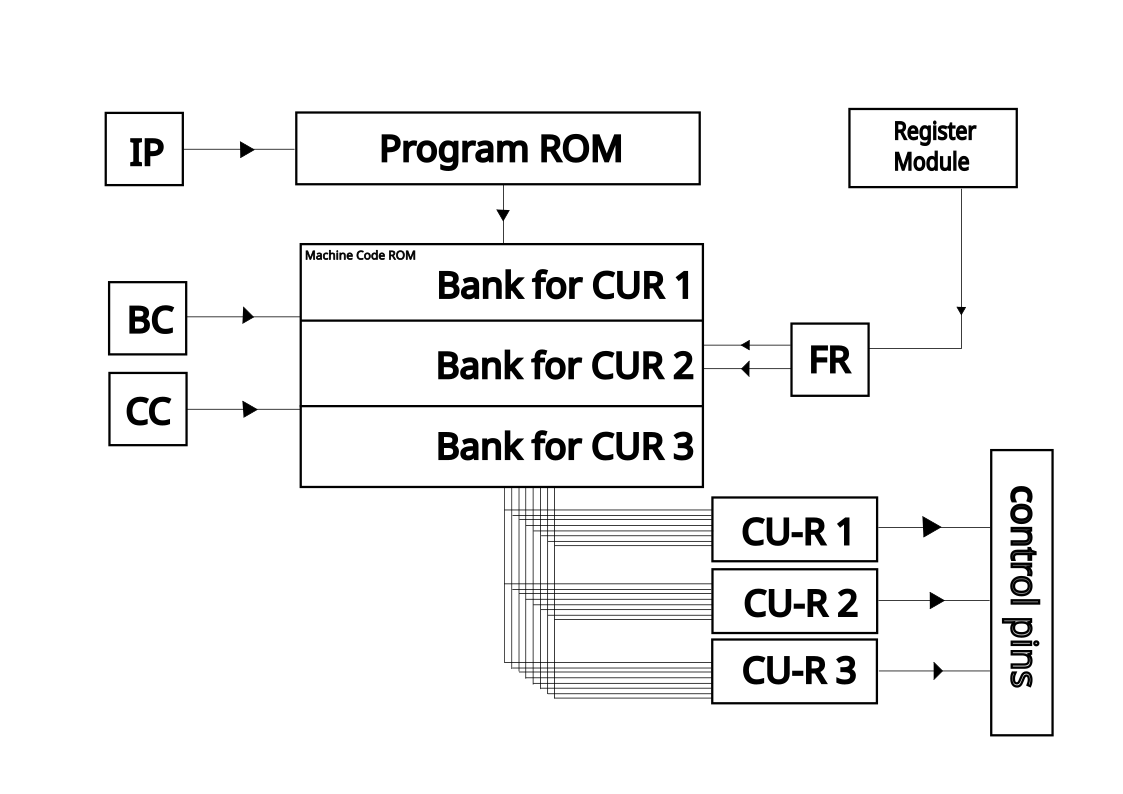
\includegraphics[width=0.9\textwidth]{img/CU}
	\caption{Control Unit Diagram}
	\label{fig:cu_diagram}
\end{figure}

Firstly, the Machine Code ROM has a certain number of address lines composed of the output of the two counters (BC and CC), flag register, and program ROM. 

As described in \ref{sec:implementation:memory:rom}, the Program ROM contains the actual executable that the processor aims to execute. Each address contains a specific sequence of bits (called instructions) that are to be loaded in the Machine Code ROM to search for and trigger the responsible physical action. Each Program ROM's instruction is referred to by the IP. To conclude, the first part of the Machine Code ROM address involves the output of the Program ROM.

The next part is counter-part, BC and CC. On each cycle, which we will describe later, the counter links to the next value and gives it up as an address line for the Machine Code ROM. As indicated in \ref{fig:bank_separation_example}, the given BC value is the two most significant bits. We will explore the importance of this configuration later. 

Flag Register contributes to the two bits of the address lines. It is necessary to get the correct value for the executable machine code from of the Machine Code ROM.

In total, we have 20 control pins. Those are pins like loading, resetting, incrementing, etc. of individual registers, counters, and modules. Because we could not store a 20-bit value stored in the ROM (Machine Code ROM), it was required to separate the value in three different ROM memory locations. We called such a location the bank with appropriate number from 1 to 3. The first third of the total number of memory of the ROM is dedicated for the bank 1, the second third - for the bank 2, and the same for the bank 3. C++-generated example you can see in the figure below:

\begin{figure}[H]
	\centering
	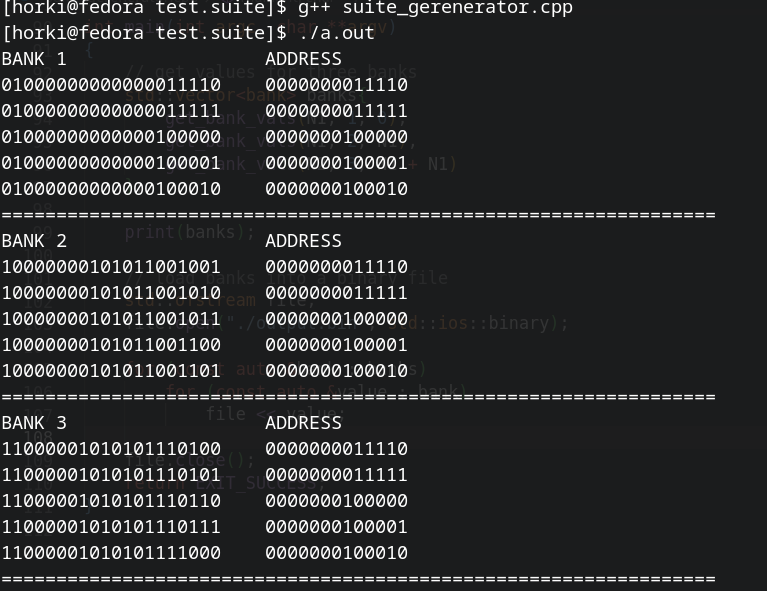
\includegraphics[width=0.9\textwidth]{img/bank_separation_example}
	\caption{Banks in the Machine Code ROM}
	\label{fig:bank_separation_example}
\end{figure}

The first two bits (most significant) are decided by BC, and are responsible for the bank selection. For example, 00 selects for the bank 1, 01 - for the bank 2, and 10 - for the bank 3. However, what would we do with 11 value\footnote{Remember, the bank counter is a 4-bit counter, thus it traverses this cycled linked-list: 00 -> 01 -> 10 -> 11 -> 00}? We deal with this problem by using all four possible cycles of the cycle counter. 

Providing a reasonable address to the Machine Code ROM, the output is the 8-bit bank value, which is a part of the entire 20-bit action that is directly connected to control pins via CURs. 

The major problem is how do we load the 20-bit values if we are restricted by 8-bit output from the Machine Code ROM? This is solved by the cycle counter, and 3-state behavior of the CURs. 

When we start the computer, the first value on CC is 00 - a so-called beginning cycle. At the same time, the value on BC is 00, thus, the first bank is selected. Remembering, that each action is edge-triggered, we can separate some number of actions during the same clock pulse: on raising and falling edge. On the raising edge, we load data from the Machine Code ROM and select the CU-R 1, because we do not want the first 8-bit of the machine code to be loaded in the CU-R 2 and CU-R 3. On the falling edge of the same pulse, we load this 8-bit value of the bank 1 in the CU-R 1; and we increase the value of counters. Now, we are on the cycle 01, where we perform absolutely the same operations, but now we select a different CU-R. The same applies for the cycle 10. After the machine code is loaded in every CU-R, we need some way to combine them all and execute, and also to set BC to 00. This all is done on the raising and falling edge of the fourth (11) cycle: enable the output of all CURs (3-state behavior), increment BC two times (10->11->00), and some minor configurations. As the last step, we execute control pins on the same clock cycle. To shed more light here, you can scrutinize the time-diagram below, and skim through an example in \ref{sec:control_unit:example}\footnote{Before it, remember that the falling edge is implemented via inverting the actual clock, so the falling edge is equal to the inverted raising edge}.


\begin{figure}[H]
	\centering
	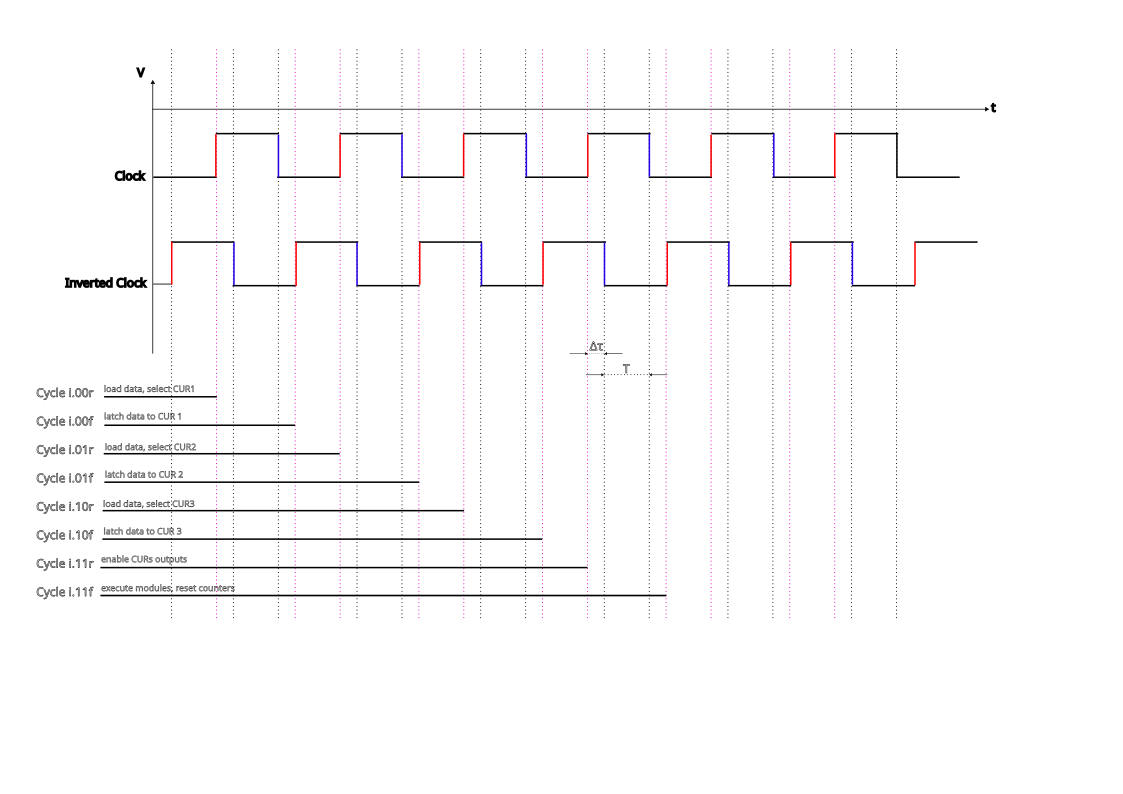
\includegraphics[width=0.9\textwidth]{img/CU_clock}
	\caption{Clock Diagram for the CU}
	\label{fig:cu_clock_diagram}
\end{figure}


\subsection{Example} \label{sec:control_unit:example}



\subsection{Performance} \label{sec:control_unit:performance}
It is overtly difficult to get an exact formula or graph for performance. Therefore, first comes a theoretical estimate/formula (see \ref{sec:control_unit:performance:theretical_estimate}), and afterward a diagram showing the speed comparison of BFCPU and an ordinary computer with *****processor******* for different programs {(see \ref{sec:control_unit:performance:comparison})}. 

\subsubsection{Theoretical Estimate} \label{sec:control_unit:performance:theretical_estimate}
Introduce new symbols:

\[\delta \tau \textmd{- inverting delay (see \ref{fig:cu_clock_diagram}).}\]

\[T \textmd{ - clock pulse period (see \ref{fig:cu_clock_diagram}).}\]

\[t_{i}^{j} \textmd{ - execution time of performing an action j in i-th component (such as D-R resetting). } \]

\[t_{max} \textmd{ - time of execution. }\]

\[N \textmd{ - number of instructions in the Program ROM. }\]

Time of execution must be less than the clock pulse period. Otherwise, a new pulse will be generated before previous commands have been still being executed. Because action of components are occurring simultaneously, only the maximum execution time is important. This results in this possible formula for the highest frequency of the clock (see \ref{sec:clock:implementation}) for the instruction k:

\[ f_{k_{max}} = \frac{1}{\delta \tau + \max{(t_{i}^{j})}} \]

This suggests the following estimate formula for the average frequency for the given program with N instructions: 

\[ <f> = \frac{1}{\frac{1}{N} \sum_{k = 1}^{N} (\delta \tau + \max{(t_{i}^{j})})} \]

However, despite the formula being given, it is quite cumbersome to check the error. This results from the fact that under given conditions, temperature, pressure, humidity, manufacturer, etc. each component might have differing execution timings. This results in the lack of data.


\subsubsection{***Processor*** Comparison} \label{sec:control_unit:performance:comparison}




